\section{Linguistic Linked Open Data} %: Building the Cloud}

Recent years have seen not only a number of approaches to provide linguistic data as Linked Data, but also the emergence of larger initiatives that aim at interconnecting these resources.
The \textbf{Open Linguistics Working Group (OWLG)}\footnote{\url{http://linguistics.okfn.org}} is an interdisciplinary network open to any individual interested in linguistic resources and/or the publication of these under an open license. The OWLG is a working group of the Open Knowledge Foundation (OKFN),\footnote{\url{http://okfn.org/}} a community-based non-profit organization promoting open knowledge (i.e., data and content that is free to use, re-use and to be distributed without restriction).
In this context, the Open Linguistics Working Group (OWLG) of the Open Knowledge Foundation (OKFN) has spearheaded the creation of 
new data and the republishing of existing linguistic resources as part of an emerging Linked Open Data (sub-) cloud of linguistic resources. 

This Linguistic Linked Open Data (LLOD) cloud is a result of a coordinated effort of the OWLG, its members and collaborating initiatives, most noteably the W3C Ontology-Lexica Community Group (OntoLex, see below) specializes in lexical-semantic resources.
As the OWLG organizes the LDL workshop series also as a vehicle to facilitate, to promote and to support this process, we would like to take the chance to unveil a revised cloud diagram on the occasion of LDL-2015.

\subsection{The LLOD Cloud}

\emph{Linguistic} Linked Open Data is defined as any kind of Linked Open Data resource considered relevant for linguistic research or Natural Language Processing. 
In March 2015, the OWLG proposed an operational definition to replace the earlier, informal use of the term `linguistically relevant'.

\subsubsection{Linguistically relevant resources}

In this context, a dataset is \textbf{linguistically relevant} if it provides or  describes language data that can be used for the purpose of linguistic research or natural language processing. Besides \emph{linguistic resources in  a strict sense} (1), this includes \emph{other linguistically relevant} resources (2) that can be used for  annotating, enriching, retrieving or classifying language resources.
\begin{enumerate}[(1)]
\item \textbf{Linguistic resources in a strict sense} are resources which have been intentionally created for the purpose of linguistic research or natural language processing, and which contain linguistic classifications, annotations, or analyses or have been used to provide such information about language data.
\item \textbf{Other linguistically relevant} resources include all other  resources used for linguistic research or natural language processing,  but not necessarily created for this purpose, e.g., large collections of  texts such as news articles, encyclopedic or terminological knowledge  or general knowledge bases such as DBpedia, or metadata collections, but only if they include incoming or outgoing links with at least one linguistic resource in a strict sense. 
\end{enumerate}

This definition is designed to provide clear-cut criteria as to whether an LOD resource can be included in the LLOD diagram, and in condition (2), it is specific to this purpose:
Condition (1) can be verified by associated publications at linguistic/NLP conferences, journals or inclusion in metadata collections such as the LREMap. 
Condition (2) can be verified by the existence of links between a resource (whose linguistic relevance is to be confirmed) and resources fulfilling condition (1).

A prototypical example for condition (1) would be a linguistics-/NLP-specific vocabulary, a dictionary with rich grammatical information or an annotated corpus, prototypical examples for condition (2) are resources which are frequently used in NLP and linguistics, but which have neither been created within these communities nor do they contain specifically linguistic information, e.g., the DBpedia.

It should be noted that condition (1) does not extend to all kinds of language resources, but limits our scope to those with \emph{annotated or analysed data}. 
A corpus with vast amounts of primary data, even if created for linguistic research, published as such and automatically converted to Linked Data, e.g., using the NLP Interchange Format
is certainly a valuable \emph{language resource}, but does not necessarily constitute a linguistic resource in a strict sense according to condition (1).

Nevertheless, it may be a linguistic resource by merits of condition (2): 
If a LOD resource does not comprise a sufficient number of links to resources that fulfill condition (1), 
it can link its annotations with terminology resources like lexvo (for language identifiers),\footnote{
	\url{http://www.lexvo.org}
} OLiA (for linguistic annotations)\footnote{
	\url{http://purl.org/olia}
}
or WordNet (for lexical senses)\footnote{
	e.g., \url{http://wordnet-rdf.princeton.edu/}
} would be sufficient for inclusion.

Linguistic \textbf{Linked} Open Data, then, comprises resources that are provided under an open license and published in conformance with the Linked Data principles as stated above.
Typically, these do not represent resources which are RDF-native, but resources that have been transformed into Linked Data. 

\subsubsection{Infrastructure and Metadata}

The official LLOD cloud diagram is hosted under \url{http://linguistics.okfn.org/resources/llod/}. 
In addition, a dynamic snapshot can be generated on-the-fly under \url{http://linguistic-lod.org}.

The LLOD cloud diagram is generated from metadata maintained at Datahub.\footnote{
	\url{http://datahub.io}
}
Currently, an alternative metadata repository specialized to linguistic resources is under development, Linghub.\footnote{
	\url{http://linghub.lider-project.eu/}
}
At the time of writing, we have initiated a process of transfer between both systems, Linghub has been populated from and is cross-linked with Datahub meta data, 
and the resources in the LLOD diagram are linked with Linghub entries. 
In the longer perspective, and after thorough review by the community, Linghub is planned to replace Datahub.
Nevertheless, this is still experimental, and we currently recommend editing and maintaining LLOD resource metadata at Datahub.

We currently classify LLOD resources into three broad groups:

\begin{description}
\item[corpora] language data (with linguistic analysis)
\item[lexical-conceptual resources] models of the concepts underlying actual language data
\item[metadata] information about languages and language resources
\end{description}

\textbf{Corpora} (blue resources in Fig.\ \ref{figI18nLOD}) are collections of language data, e.g., examples, text fragments, or entire discourses.
It should be noted here that -- in accordance with condition (1) -- a `corpus' is always understood as a linguistically analyzed resource here, the defining element are annotations.
The notion of `corpus' thus extends both to classical RDF-only approaches where annotations \emph{and} primary data are modeled in RDF \citep{burchardt2008formalising}, 
as well as to hybrid models where only annotations are provided as Linked Data, but the primary data is stored in a conventional format \citep{cassidy2010rdf}. 
In our context, it does \emph{not} extend to collections of (unanalyzed) primary data. 
At the moment, corpora in the LLOD cloud seem to be relatively rare, 
but this only reflects the fact that several corpora had to be excluded from the diagram because they were not linked yet with other LLOD data sets such as lexical resources or repositories of annotation terminology.

\textbf{Lexical-conceptual resources} (green resources in Fig.\ \ref{figI18nLOD}) focus on the general meaning of words and the structure of semantic concepts. 
These represent by far the most established and flourishing type of linguistic resources in the Linked Data context: They have been of inherent interest to the Semantic Web community, and hence a long tradition in this regard, going back to earliest attempts to integrate WordNet into the Semantic Web world \citep{gangemi2003ontowordnet}. 
In the diagram, we distinguish two types of lexical-conceptual resources, i.e., 
\emph{lexical resources} which also provide grammatical information (lexicons and dictionaries), and 
\emph{term bases} which focus on vocabulary rather than linguistics (terminologies, thesauri and knowledge bases such as YAGO and DBpedia) 
and whose origins lay outside of the stricter boundaries of linguistics or NLP. 
While the latter do not provide us with grammatical information, they formalize semantic knowledge, and in this respect, they are of immanent relevance for Natural Language Processing tasks such as Named Entity Recognition or Anaphora Resolution. 

\textbf{Metadata} (reddish resources in Fig.\ \ref{figI18nLOD}) includes resources providing information about language and language resources, 
i.e., typological databases (collections of features and inventories of individual languages, e.g., from linguistic typology), linguistic terminology repositories (e.g., grammatical categories or language identifiers), and metadata about language resources (linguistic resource metadata repositories, incl. bibliographical data).
While bibliographical data and terminology management represent classical Linked Data applications, \emph{typological databases} are a specifically linguistic resource:
Databases of features of individual languages are a particularly heterogeneous group of linguistic resources; they contain complex and manifold types of information, e.g., feature structures that represent typologically relevant phenomena, along with examples for their illustration and annotations (glosses) and translations applied to these examples (structurally comparable to corpus data), or word lists (structurally comparable to lexical-semantic resources). RDF as a generic representation formalism is thus particularly appealing for this class of resources.

LLOD resources are semiautomatically classified into these categories on the basis of tags used to describe them at Datahub.

Another type of metadata is concerned with licensing information. 
Among LLOD data sets, we encourage the use of \textbf{open} licenses. 
As defined by the Open Definition, ``openness'' refers to ``[any] piece of content or data [that] is open if anyone is free to use, reuse, and redistribute it -- subject only, at most, to the requirement to attribute and share-alike.''\footnote{\url{http://opendefinition.org}}
At the moment, this condition is not yet enforced for the diagram, but also a small number of resources (10\%=13/126) are included which are available for academic research but at the moment not under an open license.
However, legal metadata is also classified and a specific visualization can be generated with the dynamic edition of the diagram.\footnote{
	\url{http://linguistic-lod.org/llod-cloud}
}
In the longer perspective, we expect a growth of linked data resources, so that our continuous move towards increasingly rigid quality criteria may eventually exclude non-open resources from the LLOD diagram.
At the same time, however, we expect growing number of licensed linked data resources, which may give rise to a `Licensed Linked Data cloud' diagram which then takes the (pruned) LLOD diagram as its core -- but extends it to other resources relevant for academic research as well as industry partners.

\begin{figure*}[t]
 \begin{center}
% \includegraphics[width=0.97\textwidth]{images/LODLinguistics.jpg}
% \includegraphics[width=0.97\textwidth]{images/llod}
 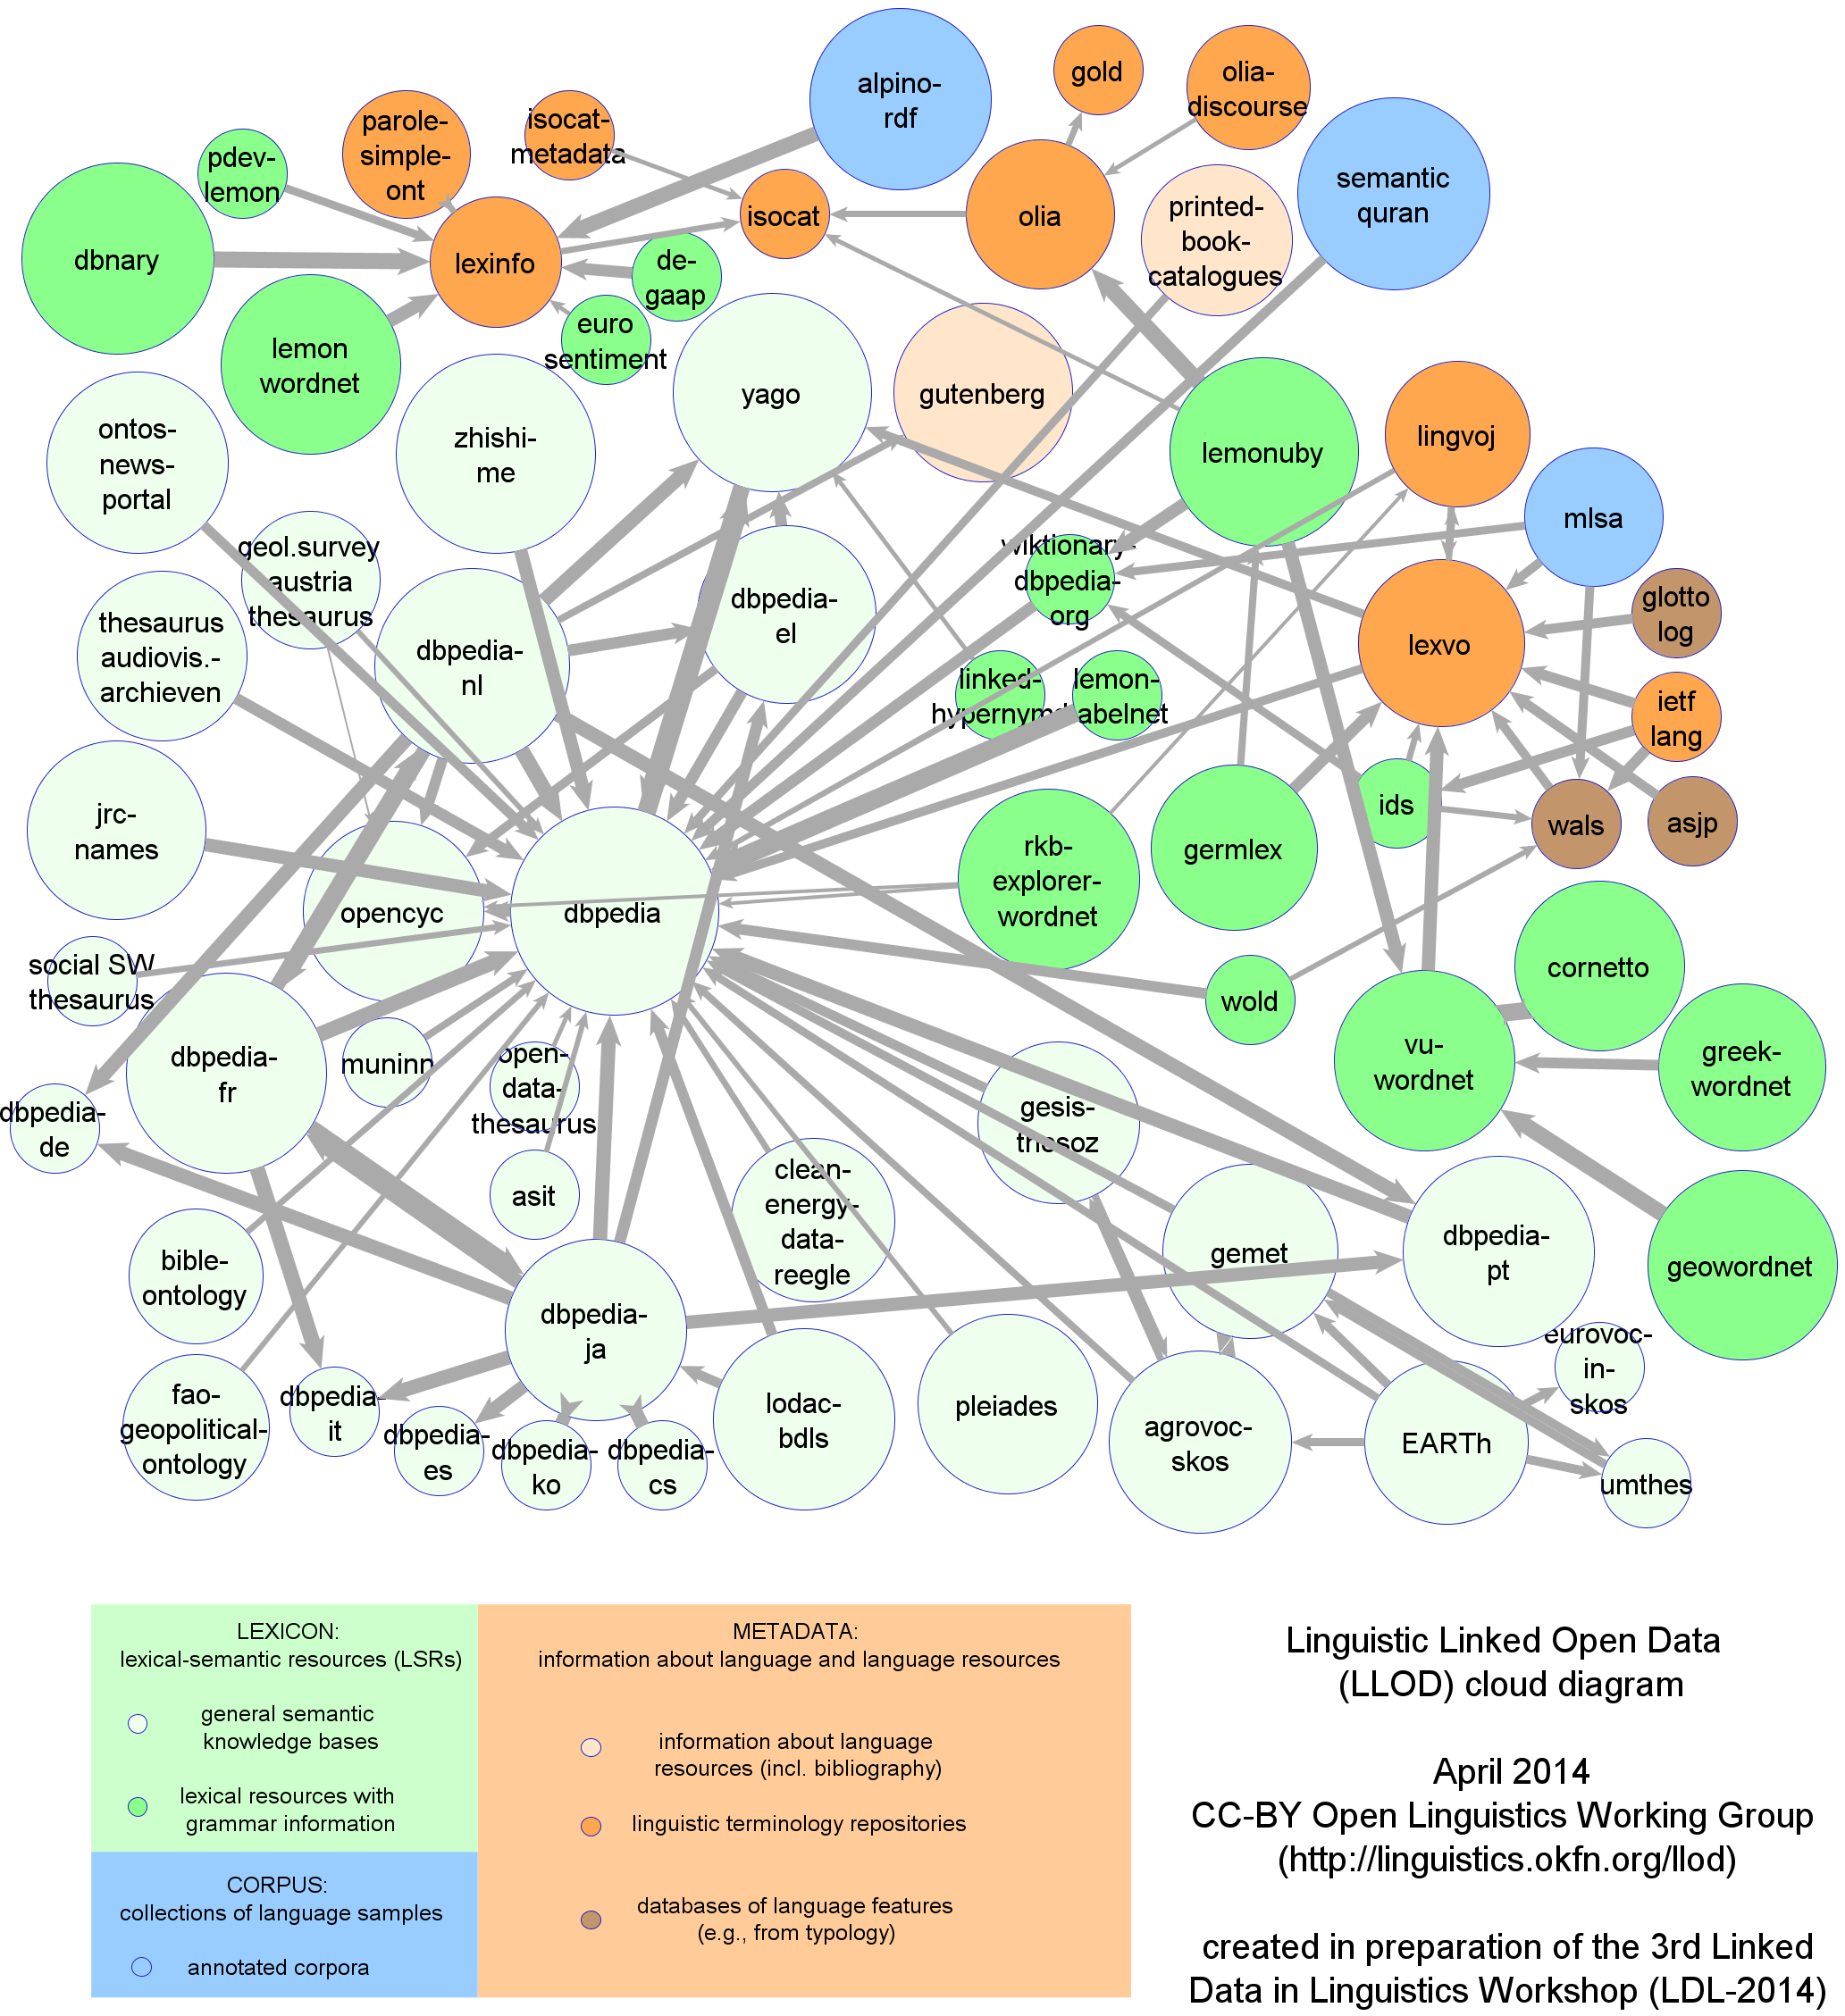
\includegraphics[width=1.0\textwidth]{llod-colored.png}
 \end{center}
\caption{Linguistic Linked Open Data cloud as of June 2015 [TO BE UPDATED]}
\label{figI18nLOD}
\end{figure*}

\subsection{Recent Developments}

Since we initiated the LDL workshop series and the LLOD cloud in 2012, we have seen a great rise of interest in the matter from the side of linguistics, Natural Language Processing and Semantic Web communities. The topic gained a lot of attention in the language resource community since the First Workshop on Linked Data in Linguistics in 2012, e.g., at LREC-2014, where Nicolatta Calzolari identified Linguistic Linked Open Data as `the new hot topic in our community' in the closing ceremony.

\paragraph{Resources} 
LREC-2014 also hosted the last instantiation of the LDL workshop series in May 2014 in Reykjavik, Iceland, which was accompanied by a datathon in orer to encourage providing (open) linguistic resources as Linked Data. 
Since then, the community has continued to gather and to convert data sets, we kept on refining our classification of language resources and encouraged others to contribute, e.g., by organizing various events on Linked Data and LLOD.
These efforts have met with success such that the number of candidate resources for the cloud has increased substantially, from 68 resources in April 2014 to 126 in June 2015. Along with this growth, we continue to enforce increased quality constraints imposed on resources in the cloud diagram. As of June 2015, we require that resources in the diagram are \emph{linguistically relevant} according to the definition given above. 
% however, this hasn't been checked
Future editions may feature increased constraints on the licensing status of LLOD resources.
% as the next step, we could eliminate non-open resources, the only major loss will be BabelNet, so the linking of everything currently connected via BabelNet only will need to be improved

\paragraph{Terminology}
For about a year, the OWLG has struggled to provide a consensus definition for LOD resources to be included in the LLOD cloud diagram, a tideous process given the great multidisciplinary character and the resulting heterogeneity of the Open Linguistics Working Group. 
In March 2015, we arrived at the definition given above which aims to combine different perspectives on linguistic resources and linked data, but nevertheless provides verifiable criteria for inclusion:
In order to be operational for industry partners and colleagues from Information Technology, the cloud diagram must not be limited to resources developed by academic circles with linguistic or NLP background (i.e., `linguistic resources' in a strict sense), but should extend to resources actively used by these groups (as well as others interested in this kind of material. We thus require resources to be `linguistically relevant' rather than being inherently `linguistic', with the definition as given above. 

On this basis, we are currently working towards aligning the resource classification with those of metadata repositories such as META-SHARE and LREMap.

\paragraph{Infrastructure}
For generating the diagram, we mostly rely on the metadata as provided by Datahub.io, so only datasets are considered whose links with other LLOD data sets are explicitly documented there.
In the context of the European LIDER project and LD4LT W3C Community Group, a linked-data-based metadata repository for linguistic resources has been developed, Linghub, which is currently populated from Datahub as well as from the LREMap,\footnote{\url{http://www.resourcebook.eu/}} META-SHARE\footnote{\url{http://www.meta-net.eu/meta-share}} and the CLARIN Virtual Language Observatory.\footnote{
	\url{http://catalog.clarin.eu/vlo/}
}
Although Datahub is sill being recommended for entering and managing metadata, the transfer from Datahub to Linghub is conducted under semiautomatic control, so that a certain level of quality can be assured. A stricter validation routine is envisioned. % status? do we still test whether URLs are alive?

Furthermore, we set up a website dedicated to linguistic linked open data, \url{linguistic-lod.org}, where \emph{dynamic versions} of the diagram are hosted as well as any information about the current and future LDL workshops. This website is going to replace the current LLOD-related pages at the OWLG website and wiki, which will continue to be used for community management and non-LLOD-related activities.

\paragraph{Community}
Since Linked Data has been declared as the new hot topic in the language resource community at LREC-2014, interest sparked and we have seen a number of events dedicated to the topic, most of them with participation of OWLG members. 
Among others, this includes 
the 2nd Workshop on Multilingual Linked Open Data for Enterprises (MLODE-2014, Sep 2014, Leipzig, Germany), 
the 1st NLP\&DBpedia Workshop (Oct 2014, Riva del Garda, Trentino, Italy), 
the 4th Workshop on the Multilingual Semantic Web (MSW-2015, Jun 2015, Portoroz, Slovenia),
the 12th EUROLAN Summer School (EUROLAN-2015, Jul 2015, Sibiu, Romania, dedicated to Linguistic Linked Open Data),
the Workshop on the Development of Linguistic Linked Open Data Resources for Collaborative Data-Intensive Research in the Language Sciences at the LSA Summer Institute 2015 (LLOD-LSA 2015, Jul 2015, Chicago),
as well as upcoming events like 
the 2nd Workshop on Natural Language Processing and Linked Open Data (NLP\&LOD-2015, Sep 2015, Hissar, Bulgaria) and 
the 2nd NLP\&DBpedia Workshop (Oct 2015, Bethlehem, Pennsylvania).
In addition, Linguistic Linked Open Data has been subject to several hackathons, resp., datathons,
including LLOD-specific hackathons collocated with MLODE-2012 and MLODE-2014, and the 1st Summer Datathon on Linguistic Linked Open Data (SD-LLOD-15, Jun 2015, Cercedilla, Spain), 
but also events with broader scope such as the 2015 $\{$Cod1ng Da V1nc1$\}$ cultural hackathon (Apr/Jul 2015, Berlin, Germany)\footnote{
	\url{http://codingdavinci.de/english-infos/}
}
where typological data from the LLOD cloud has been used for developing an edutainment application.

Different community groups established themselves, including the 
Open Linguistics Working Group of the Open Knowledge Foundation (OWLG, founded Oct 2010)\footnote{
	\url{http://linguistics.okfn.org/}
}
and the W3C Community and Business Groups on Ontology-Lexica (OntoLex, founded Jan 2012)\footnote{
	\url{https://www.w3.org/community/ontolex/}
}
Best Practices for Multilingual Linked Open Data (BP-MLOD, founded Jun 2013)\footnote{
	\url{https://www.w3.org/community/bpmlod/}
} and Linked Data for Language Technologies (LD4LT, founded Jan 2014).\footnote{
	\url{https://www.w3.org/community/ld4lt/}
}
Among these, the W3C groups take a relatively narrow focus on specific aspects of Linked Data for NLP, whereas the OWLG provides an umbrella comprising these and other activities in relation to open linguistic resources as well providing a forum for interested researchers, data providers and user communities from linguistics who would not normally work in the context of the W3C. 
For general information, the OWLG and its mailing list\footnote{
	\url{https://lists.okfn.org/mailman/listinfo/open-linguistics}
} would be a good point of contact for anyone interested in the matter. 
The OWLG overlaps with the W3C Community Groups in terms of the persons involved, and recent developments from the W3C groups are regularly reported at OWLG meetings.
Specific technical issues and business cases are subject to the W3C community groups.

Following a trend already observed in 2014, and partially due to the progress of the OntoLex Working Group, the fastest-growing class of LLOD resources are lexical-conceptual resources. 
Partially, this reflects the increasing reception of the \emph{lemon} vocabulary in the community, but also the activities of the W3C Ontology-Lexica Community Group (OntoLex). The OntoLex group is not only closely collaborating with the OWLG, but both also have a considerable overlap in terms of their members, and as usual since LDL-2013, several organizers of LDL-2015 are active in both groups.
While the OWLG is interested in open linguistic resources in general, the OntoLex group takes a specific focus on lexical resources, culminating in the proposal of a common model for machine-readable lexicons in RDF, the \emph{lemon} model.\footnote{
	\url{http://lemon-model.net}
}

\paragraph{Vocabularies}

Already at LDL-2014, we have seen a standardization of vocabularies used for modelling LLOD resources, most noteably lemon and lexinfo (for lexical resources) as well as lexvo (for language identifiers). The resulting degree of interoperability and visibility arising from the use of shared vocabularies is certainly one of the most concrete achievements of the community activities we aimed to initiate with forming the OWLG, preparing the LLOD diagram and conducting workshops at linguistic, NLP and IT conferences.

At the same time, extensions and limitations of established vocabularies are being noted and an active development cycle has been started, e.g., pertaining possible extensions of lemon (cf. the contribution by Lee and Hsieh in this volume) or NLP Interchange Format (NIF, cf. S\'{a}nchez-Rada, Iglesias and Gil, in this volume). 
It should be noted that such proposals do not indicate deficits of the existing vocabularies, but rather arise from their adaptation by a novel community with novel challenges which were out of the original use case. As such, NIF was designed as a format for NLP annotations generated on the fly, not linguistic corpora, and lemon was not designed as a generic vocabulary for lexical resources, but for the specific task of adding lexical information to an existing ontology. 
The extension of vocabularies and the development of downward-compatible extensions will be one of the key issues of the future development of LLOD and the communities behind.
 
\subsection{Organizing LDL-2015}

The LDL workshop series and LDL-2015 are organized by the Open Linguistics Working Group 
to bring together researchers from various fields of linguistics, NLP, and IT to present and discuss principles, case studies, and best practices for representing, publishing and linking linguistic data collections, and aims to facilitate the exchange of technologies, ideas and resources across discipline boundaries, that (to a certain extend) find a material manifestation in the emerging LLOD cloud.

LDL-2015, collocated with ACL-IJCNLP 2015, the 53rd Annual Meeting of the Association of Computational Linguistics and the 7th Joint Conference on Natural Language Processing of the Asian Federation of Natural Language Processing in July 2015 in Beijing, China, is the fourth workshop on Linked Data in Linguistics following LDL-2012 (March 2012 in Frankfurt am Main, Germany), LDL-2013 (Sep 2013 in Pisa, Italy),
and LDL-2014 (May 2014, Reykjavik, Iceland), as well as more specialized events such as the workshops on Multilingual Linked Open Data for Enterprises (MLODE-2012: Sep 2012 in Leipzig, Germany, MLODE-2014: Sep 2014 in Leipzig, Germany), and Natural Language Processing and Linked Open Data (NLP\&LOD-2013: Sep 2013 in Hissar, Bulgaria), and the theme session on Linked Data in Linguistic Typology (at the 10th Biennial Conference of the Association for Linguistic Typology, ALT-2013, Aug 2013 in Leipzig, Germany), as well as presentations, panels and informal meetings at various conferences.

LDL-2015 is organized by the \emph{Open Linguistics Working Group} (OWLG) of the Open Knowledge Foundation. Since its foundation in October 2010, the OWLG has grown steadily. One of our primary goals is to attain openness in linguistics through:

\begin{enumerate}
\item Promoting the idea of open linguistic resources,
\item Developing the means for the representation of open data, and
\item Encouraging the exchange of ideas across different disciplines.
\end{enumerate}

The OWLG represents an open forum for interested individuals to address these and related issues.
At the time of writing, the group consists of about 150 	% that's a very conservative estimate, as of June 27, 2015, we have 217 subsribers 
															% (but there are a few duplicates, a few pseudo-addresses with purely technical 
															% function, and 3 unsubscriptions)
															% for LDL-2014, we estimated 130 actual people from a total of 185 subscribers, i.e., 70%
															% for LDL-2015, we thus estimate 152 people 
people from more than 20 									% 20 was an estimate from 2013 (!), not checked
different countries.
As our group is continuously growing, it also remains heterogeneous, and includes people from library science, typology, historical linguistics, cognitive science, computational linguistics, and information technology; the ground for fruitful interdisciplinary discussions has been laid out.
One concrete result emerging out of collaborations between a large number of OWLG members is the LLOD cloud as already sketched above.

The emergence of the LLOD cloud out of a set of isolated resources was accompanied and facilitated by a series of \textbf{workshops and publications} organized by the OWLG as sketched above. 
Plans to create a LLOD cloud were first publicly announced at LDL-2012, and subsequently, a first instance of the LLOD materialized as a result of the MLODE-2012 workshop, its accompanying hackathon and the data postproceedings that appeared as a special issue of the Semantic Web Journal (SWJ). 
The 4th Workshop on Linked Data in Linguistics continues this series of workshops, and in order to further contribute to the integration of the field, their organizers again involved members of both the OWLG and the W3C Ontology-Lexica Community Group.

The \textbf{Ontology-Lexica Community (OntoLex) Group}\footnote{\url{http://www.w3.org/community/ontolex}} was founded  in September 2011 as a W3C Community and Business Group. It aims to produce specifications for a lexicon-ontology model that can be used to provide rich linguistic grounding for domain ontologies.
Rich linguistic grounding includes the representation of morphological, syntactic properties of lexical entries as well as the syntax-semantics interface, i.e., the meaning of these lexical entries with respect to the ontology in question. An important issue herein will be to clarify how extant lexical and language resources can be leveraged and reused for this purpose. As a byproduct of this work on specifying a lexicon-ontology model, it is hoped that such a model can become the basis for a web of lexical linked data: a network of lexical and terminological resources that are linked according to the Linked Data Principles forming a large network of lexico-syntactic knowledge.

Like LDL-2014, LDL-2015 is supported by the EU Projects LIDER and QTLeap:
The project \textbf{Linked Data as an Enabler of Cross-Media and Multilingual Content Analytics for Enterprises Across Europe} (LIDER) aims to provide an 
ecosystem for the establishment of linguistic linked open data, as well as media resources metadata, for a free and open exploitation of such resources in 
multilingual, cross-media content analytics across Europe. 
The project \textbf{Quality Translation with Deep Language Engineering Approaches} (QTLeap) explores novel ways for attaining machine translation of higher quality that are opened by a new generation of increasingly sophisticated semantic datasets (including Linked Open Data) and by recent advances in deep language processing.

To accomodate the importance of multilinguality and semantically-oriented NLP that we encounter in the community as well as these initiatives, LDL-2014 takes a focus on Multilingual Knowledge Resources and Natural Language Processing, although contributions on Linked Data emphasising other aspects of linguistics or NLP were explicitly encouraged.